\subsection{Conversor Digital para Analógico}
\subsubsection{Introdução}
O inversor de frequência escolhido para o projeto pode ser controlado usando uma referência analógica de tensão ou de corrente para aferir a velocidade do motor a ser controlado. Foi definido que será usada a referencia analógica de tensão pois a mesma e controlada por uma tensão que varia de 0 a 10V enquanto a referencia por corrente se da dentro de um intervalo de 4 a 20mA, o circuito de condicionamento de sinais para o intervalo de tensão acima e mais simples e robusto do que o de corrente baseado no microprocessador escolhido (MSP430). O microcontrolador não possui uma saída de tensão analógica porém possui saídas capazes de serem utilizadas com PWM (Pulse Width Modulation), usando um simples circuito de conversão de sinais se torna possível converter uma saída de tensão digital de PWM que varia de 0 a 3.3V (tensão máxima e mínima de saída do MSP430) em uma saída de tensão analógica de 0 a 10V.
\subsubsection{PWM}
Um sinal PWM é formado por uma série de pulsos de amplitude e frequência fixas porém com largura dos pulsos variável. Assim como é possível transmitir um sinal analógico por primeiramente modulando o sinal em uma onda portadora e depois removendo a portadora e ficando apenas com o sinal, também é possível transmitir uma tensão analógica modulada em uma portadora digital. Essa tensão analógica pode ser facilmente extraída do sinal modulado um usando um filtro passa-baixas.
\begin{figure}[htbp]
	\centering
	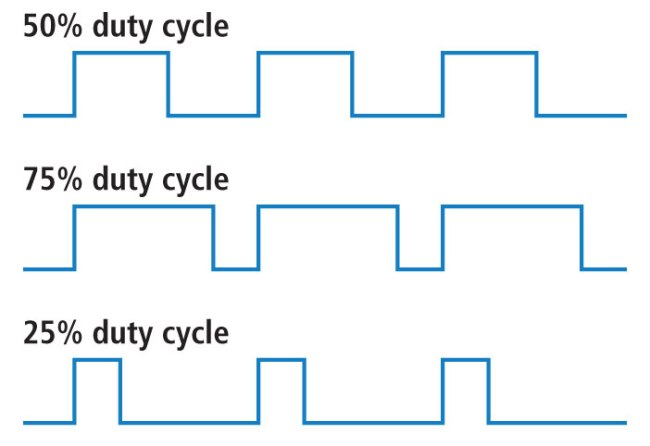
\includegraphics[scale=0.3]{figuras/duty_cycle.jpg}
	\caption{Duty Cycle}
	\label{duty_cycle}
\end{figure}
Em PWM, o tempo em que o sinal fica em nível lógico alto ou baixo não costuma ser muito usado, o mais comum é classificar o sinal de acordo com seu duty-cycle. A relação entre duty-cycle, amplitude e tensão nominal de saída do DAC se torna bem intuitiva. No domínio da frequência, um filtro passa-baixas suprime componentes de alta frequência, consequentemente no domínio do tempo isso acaba "amaciando" o sinal e de certa forma tirando uma media do sinal. Filtrar um sinal PWM com um filtro passa-baixas extrai seu valor médio de tensão. Se por exemplo o duty-cyle de um sinal for 50\% com máximo e mínimo respectivamente em 5 e 0V, após o sinal ser passado pelo filtro o sinal de saída ira possuir uma saída de 2.5V.

\begin{equation}\label{calc-duty-cycle}
	D=\frac{ PW }{ T } \cdot 100 \%
\end{equation}

Na Equação \ref{calc-duty-cycle}, D é o valor do duty cyle em percentagem, PW a largura do pulso e T o período total do sinal.

\begin{equation}\label{calc-analog-voltage}
	V_{out}=\frac{ Pw }{ T } \cdot V_{max}
\end{equation}

A Equação \ref{calc-analog-voltage} calcula a tensão de saída aproximada do sinal após o filtro passa-baixas. Na mesma $V_{out}$ é a tensão de saída, PW a largura do pulso e T o período total do sinal e $V_{max}$ é a tensão do sinal PWM quando em nível lógico alto.

\subsubsection{Filtro passa-baixas}

Existem duas condições a serem consideradas no projeto do filtro passa-baixas: O tempo de estabilização e o ripple. Tempo de estabilização é o tempo que o sinal leva para chegar ao nível analógico desejado, já o ripple é o ruído residual da filtragem do sinal do saída. Uma frequência de corte baixa gera um sinal com pouco ripple porém aumenta o tempo de estabilização, consequentemente uma frequência de corte mais alta produz um ripple muito grande e um tempo de estabilização curto. O que deve ser feito é escolher uma frequência de corte que gera um ripple menor que a resolução da entrada analógica do inversor de frequência (vale lembrar que resolução é a menor variação de tensão que o dispositivo pode ler). \\

As especificações para projeto do filtro conversor são:

\begin{itemize}
	\item Frequência PWM de entrada = 100KHz
	\item Resolução da entrada do inversor (ripple máximo) = 9.76mV
	\item Tempo de estabilização = 0.1s
	\item Ganho de Tensão = 3
\end{itemize}

O circuito a ser usado será o da Figura \ref{active-lpf}:

\begin{figure}[htbp]
	\centering
	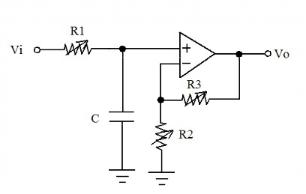
\includegraphics[scale=0.3]{figuras/lpf.jpg}
	\caption{Filtro passa-baixas ativo}
	\label{active-lpf}
\end{figure}

A frequência de corte para o filtro é dada pela Equação \ref{cuttof-frequency}

\begin{equation}\label{cutoff-frequency}
	f_{c}=\frac{ 1 }{ 2 \Pi \cdot R_{1}\cdot C } \cdot V_{max}
\end{equation}

Os resistores $R_{2}$ e $R_{3}$ controlam o ganho do filtro que é dado pela Equação \ref{ganho_alpf}

\begin{equation}\label{calc-analog-voltage}
	G= 1 + \frac{ R_{3} }{ R_{2} }
\end{equation}

Foram usados os seguintes componentes para o circuito:

\begin{itemize}
	\item $R_{1}=10k\Omega$
	\item $R_{2}=100k\Omega$
	\item $R_{3}=200k\Omega$
	\item C=1uF
\end{itemize}

Esse circuito gera uma frequência de corte de aproximadamente 16Hz, um ripple de 2.4mV, um tempo de estabilização de 0.02s e um ganho de tensão igual a 3. Dessa forma atende todas os requisitos de funcionamento. A Figura \ref{filter_out} mostra a saída sem ripple.

\begin{figure}[htbp]
	\centering
	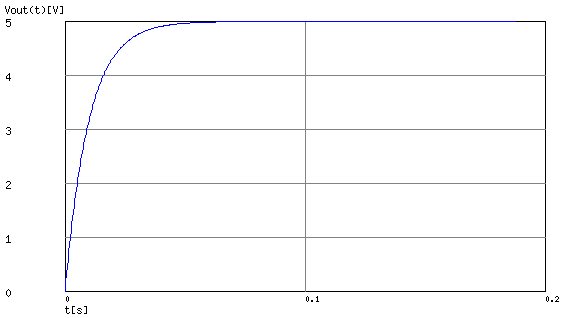
\includegraphics[scale=0.3]{figuras/ripple-lpf.jpg}
	\caption{Gráfico TensãoxTempo filtro passa baixas}
	\label{filter_out}
\end{figure}
